% !TeX program = pdflatex
% !TeX encoding = UTF-8
\documentclass[sigconf,nonacm,screen]{acmart}
\usepackage{styles/course-report}
\graphicspath{{figures/}}

\title[图像聚类与工业缺陷检测]{图像聚类与工业缺陷检测\texorpdfstring{\\}{ · }数据挖掘导论课程报告（任务1与任务2）}
% 填写三位组员姓名、学号和院系后重新编译。
\author{组员一（待填写）}
\affiliation{\institution{学号待填写}\city{院系待填写}}
\author{组员二（待填写）}
\affiliation{\institution{学号待填写}\city{院系待填写}}
\author{组员三（待填写）}
\affiliation{\institution{学号待填写}\city{院系待填写}}
\renewcommand{\shortauthors}{}



\makeatletter
\def\@ACM@checkaffil{}%
\makeatother

\begin{abstract}
本报告使用课程提供的工业图像完成两项实验。图像聚类在冻结的 ResNet-50 特征中融合图像语义、纹理和颜色，随后在局部尺度近邻图上做谱聚类。600 张图像全部与参考类别匹配，调整兰德指数和归一化互信息均为 1.000。异常检测将图像块到正常样本库的最近邻距离与整图支持向量机的判别分数结合。融合权重和阈值由训练集五折验证确定。榛子和拉链两类的独立测试集共 102 张图像，融合模型全部判对，两类的 AUROC、AP 和 F1 均为 1.000。对照实验比较了特征表示、聚类方法和两个异常检测分支。
\par\noindent\textbf{关键词}\quad 图像聚类、谱聚类、异常检测、最近邻、支持向量机
\par\medskip
{\normalfont\zihao{5}\noindent\textbf{Abstract}\quad
We study image clustering and industrial anomaly detection on the supplied course datasets.
Locally scaled spectral clustering combines semantic, texture, and colour features. It recovers all six reference classes across 600 images.
For anomaly detection, we combine nearest-neighbour scores from a normal patch bank with image-level SVM scores.
Five-fold validation on the training set determines the fusion and thresholds.
The detector classifies all 102 held-out hazelnut and zipper images correctly, with AUROC, AP, and F1 of 1.000 for each product.
\par\noindent\raggedright\textbf{Key words}\quad image clustering, spectral clustering, anomaly detection, nearest neighbours, support vector machine\par}
\end{abstract}

\begin{document}
\maketitle

\section{引言}
课程绪论把聚类表述为根据特征空间的距离划分样本，把异常检测表述为从正常行为中识别有实际意义的偏离\cite{courseintro}。在本次作业中，第一项任务需要区分电缆、瓷砖等外观差异较大的产品，第二项任务需要在同种产品内部识别缺陷。前者关注整图的相似性，后者还要保留缺陷附近的局部特征。

两项实验使用作业指定数据与划分。读入时只枚举实际图像目录下的 PNG 文件。聚类集原始分辨率为 $800^2$ 至 $1024^2$ 像素，异常检测集均为 $1024\times1024$ 像素。对解码后的 RGB 像素计算 SHA-256，聚类集无完全重复图像，两类异常检测数据的训练集和测试集之间也无像素完全相同的图像。该核验只覆盖精确重复。实验使用 Python 3.12、PyTorch 2.5.1 和 scikit-learn 1.9.1，在 CPU 上运行，主随机种子设为 2026。

\section{任务1\quad 图像无监督聚类}
\label{sec:task1}
\subsection{问题描述与定义}
设课程图像集合为 $\mathcal X=\{x_i\}_{i=1}^{600}$。题目给定簇数 $K=6$，求互不重叠且覆盖 $\mathcal X$ 的非空簇 $\{C_k\}_{k=1}^K$。簇编号可任意置换，算法不使用类别名称、逐图类别标签或每簇容量约束。每图输出簇编号 $z_i\in\{1,\ldots,K\}$。训练阶段只读取像素，图结构和超参数据此确定。课程标签文件仅在评估阶段读入。

\subsection{图像特征表示}
将图像转成 RGB，用双线性插值缩放到 $224\times224$。输入网络前用 ImageNet 通道均值 $(0.485,0.456,0.406)$ 与标准差 $(0.229,0.224,0.225)$ 归一化，冻结 ImageNet 预训练的 ResNet-50（\texttt{IMAGENET1K\_V2} 权重）\cite{he2016,torchvisionweights}。卷积与池化的作用可参照课程第6章\cite{coursedeep}。将 \texttt{layer3}、\texttt{layer4} 的每个通道做全局均值池化，保留瓶口、药片等物体的整图信息。用 \texttt{layer2}、\texttt{layer3} 的通道标准差描述特征响应的空间起伏。颜色块由每通道 16 桶的归一化直方图和 $8\times8$ 网格的分块 RGB 均值组成，可补充皮革和瓷砖等类别的外观差异。

按课程特征工程中尺度归一化的思路\cite{coursefeat}，对每个非负块先逐元素开平方，再做 $\ell_2$ 归一化，记作 $\widehat{\vect f}_b$。拼接时用 $\sqrt{w_b}$ 缩放，得到
\begin{equation}
 \vect z=[\sqrt{w_b}\,\widehat{\vect f}_b]_b,
 \qquad
 \|\vect z_i-\vect z_j\|_2^2
 =\sum_b w_b\|\widehat{\vect f}_{ib}-\widehat{\vect f}_{jb}\|_2^2 .
\end{equation}
五块权重依次为 $0.32,\ 0.48,\ 0.08,\ 0.07,\ 0.05$，对应两个均值块、两个标准差块和颜色块，共 4\,848 维。均值块占八成，以整图语义为主。纯深度对照只使用两个均值块，权重为 $0.4$ 和 $0.6$。手工对照使用颜色块和灰度差分，两者权重为 $0.8$ 和 $0.2$。差分在横向和纵向各取间隔 $1,2,4,8,16$ 像素，汇总每组绝对差值的均值和标准差，再逐维标准化并按行归一化。

\subsection{方法}
物体、材料纹理和拍摄背景各有变化。全局 K-means 依赖样本到质心的距离，谱聚类则可以沿近邻图发现由多段局部邻域连成的簇。在本实验中，用两点间欧氏距离 $d_{ij}$ 寻找每图的 $h$ 个近邻。若一方是另一方的近邻，就保留这条无向边。参考局部尺度核\cite{zelnik2004}，以样本到第 $h$ 个近邻的距离为 $\sigma_i$，令
\begin{equation}
 W_{ij}=\exp\!\left(
    -\frac{d_{ij}^2}{\max(\sigma_i,\epsilon)\max(\sigma_j,\epsilon)}
                         \right),
\end{equation}
其中 $\epsilon=10^{-6}$。非邻接点对和对角元素的权重置零。

令 $D_{ii}=\sum_j W_{ij}$。归一化拉普拉斯矩阵 $L=I-D^{-1/2}WD^{-1/2}$ 用于求解下面的谱松弛问题\cite{ng2001}。
\begin{equation}
 \min_{U^\top U=I_K}\operatorname{tr}(U^\top L U).
\end{equation}
取 $L$ 最小的六个特征值对应的特征向量，逐行归一化后用 K-means 分组。对照包括手工与深度特征的 K-means、融合特征的 K-means 和 Ward 层次聚类，以及固定 $h=16$ 的纯深度谱聚类。K-means 使用 30 次 K-means++ 初始化。

邻域大小扫描 $\{8,12,16,24,32\}$。先排除连通分量超过 $K$ 的图，再选融合特征空间轮廓系数最高的划分。轮廓系数相同则比较谱间隙 $\lambda_7(L)-\lambda_6(L)$。对 $n$ 张图和 $d$ 维特征，当前稠密实现计算两两距离用时 $O(n^2d)$，图及距离矩阵使用 $O(n^2)$ 内存，稠密谱分解的最坏时间复杂度为 $O(n^3)$。

\subsection{实验结果分析}
利用匈牙利算法在混淆矩阵上寻找簇与类别的一一对应，得到匹配准确率 ACC。调整兰德指数（ARI）按样本对衡量分组的一致性并校正随机一致，归一化互信息（NMI）衡量两个划分共享的信息量。两者可以直接比较参考类别和簇编号。所有对照共用融合特征空间计算轮廓系数，以便比较同一距离定义下的簇内紧密度和簇间分离度。

\begin{table}[tbp]
 \caption{聚类对照结果（600 张图像）}
 \label{tab:clustering}
 \centering
 \begin{tabular}{@{}lrrrr@{}}
 \toprule
 方法 & ACC & ARI & NMI & 轮廓系数 \\
 \midrule
 手工 K-means & 1.000 & 1.000 & 1.000 & 0.656 \\
 深度 K-means & 1.000 & 1.000 & 1.000 & 0.656 \\
 融合 K-means & 1.000 & 1.000 & 1.000 & 0.656 \\
 融合 Ward & 1.000 & 1.000 & 1.000 & 0.656 \\
 深度谱聚类 & 1.000 & 1.000 & 1.000 & 0.656 \\
 融合谱聚类 & 1.000 & 1.000 & 1.000 & 0.656 \\
 \bottomrule
 \end{tabular}
\end{table}

五种近邻图都得到六个各含 100 张图像的连通分量，轮廓系数均为 0.6559。$h=32$ 的谱间隙最大，为 0.2889，故选为主结果。十次种子复算的 45 对划分之间，ARI 的均值和最小值均为 1.000。图\ref{fig:cluster-results}展示事后匹配的混淆矩阵和融合特征的二维 PCA 投影，前两个主成分合计解释 47.6\% 的方差。聚类使用完整特征计算距离。

\begin{figure*}[t]
 \centering
 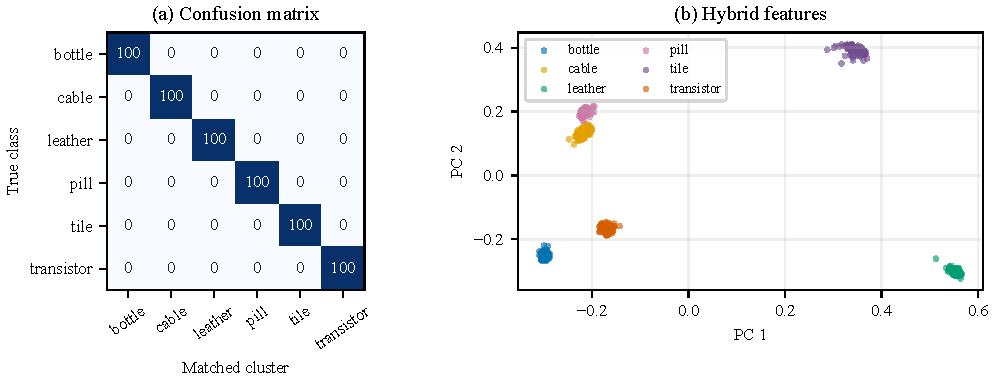
\includegraphics[width=.82\textwidth]{cluster_diagnostics}
 \caption{混淆矩阵与融合特征的 PCA 投影。散点颜色按事后匹配的簇名称标注}
 \Description{The confusion matrix contains six diagonal cells of 100. The first two principal components display the 600 images coloured by cluster.}
 \label{fig:cluster-results}
\end{figure*}

表\ref{tab:clustering}中的各方法给出同一划分，说明本数据中的形状、背景和纹理已形成很强的类别差异。图\ref{fig:cluster-exemplars}给出每簇靠近融合特征中心的图像。电缆、瓶口和药片有不同的主体轮廓，皮革和瓷砖则在色彩及细纹上有明显区别。手工特征 K-means 因此也是这个数据集上的低成本方案。本实验使用题目给定的 $K$，结果反映对这 600 张图像的聚类质量。是否能自动发现类别数，或处理背景变化和外观相近的产品，有待额外数据检验。

\begin{figure*}[t]
 \centering
 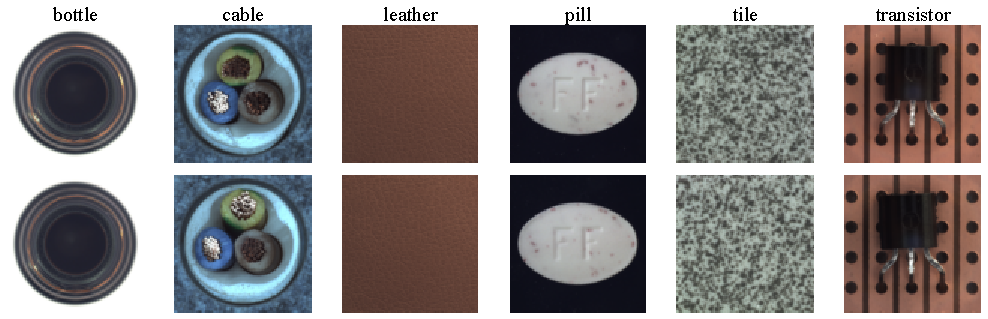
\includegraphics[width=.81\textwidth]{cluster_exemplars}
 \caption{每个簇中距其融合特征中心最近的两张图像}
 \Description{Two images each of bottles, cables, leather, pills, tiles, and transistors.}
 \label{fig:cluster-exemplars}
\end{figure*}


\section{任务2\quad 图像异常检测}
\label{sec:task2}
\subsection{问题描述与定义}
当产品类别 $c\in\{\text{hazelnut},\text{zipper}\}$ 已知时，给定该类训练集 $\mathcal D_c=\{(x_i,y_i)\}$，其中 $y=0$ 表示正常，$y=1$ 表示异常。目标是为待测图像 $x$ 学习异常分数 $s_c(x)$，分数越大越倾向于异常。按 $\widehat y=\mathbf 1[s_c(x)\ge t_c]$ 产生图像级判定，其中 $t_c$ 由训练集确定。训练中正常与异常样本之比为 $4:1$，分别按产品训练。该任务的标签是图像级，局部热图仅用于观察模型响应。

\begin{table}[H]
 \caption{异常检测数据划分}
 \label{tab:anomaly-data}
 \centering
 \begin{tabular}{@{}lrrrr@{}}
 \toprule
 产品 & 训练正常 & 训练异常 & 测试正常 & 测试异常 \\
 \midrule
 榛子 & 200 & 50 & 40 & 15 \\
 拉链 & 200 & 50 & 32 & 15 \\
 \bottomrule
 \end{tabular}
\end{table}

训练沿用课程划分（表\ref{tab:anomaly-data}）。公开 MVTec AD 提供了工业外观检测的实验背景\cite{bergmann2019}，本报告的结果对应课程发放的类别、样本与划分。测试集标签在模型、阈值和逐图分数固定后用于计分。

\subsection{图像特征表示}
榛子的小孔和拉链的不连续均可能只占很小面积。将原图双线性缩放至 $384\times384$，保持 RGB 通道和整幅视野。沿用任务1的 ImageNet 通道归一化和冻结网络。对整图分支，以 \texttt{layer2} 和 \texttt{layer3} 的通道均值及标准差、\texttt{layer4} 的通道均值、以及颜色块表示图像。按任务1的方法做开平方、分块归一化与加权拼接，六个权重依次为 $0.18,\allowbreak 0.12,\allowbreak 0.22,\allowbreak 0.13,\allowbreak 0.25,\allowbreak 0.10$，特征总维数为 5\,360。

对局部分支，从网络的前三层残差阶段取特征图。先做 $3\times3$ 局部均值池化，再对齐到 $24\times24$ 网格。每层、每位置的通道向量分别作 $\ell_2$ 归一化。将浅中层（第1、2阶段）和中层（第2、3阶段）分别拼接成两套图像块特征。各用固定种子的高斯随机矩阵投影为 48 维，再做 $\ell_2$ 归一化，以降低正常图像块检索的内存和计算开销。浅层保留相邻纹理和边缘，中层覆盖更大感受野。

\begin{figure*}[t]
 \centering
 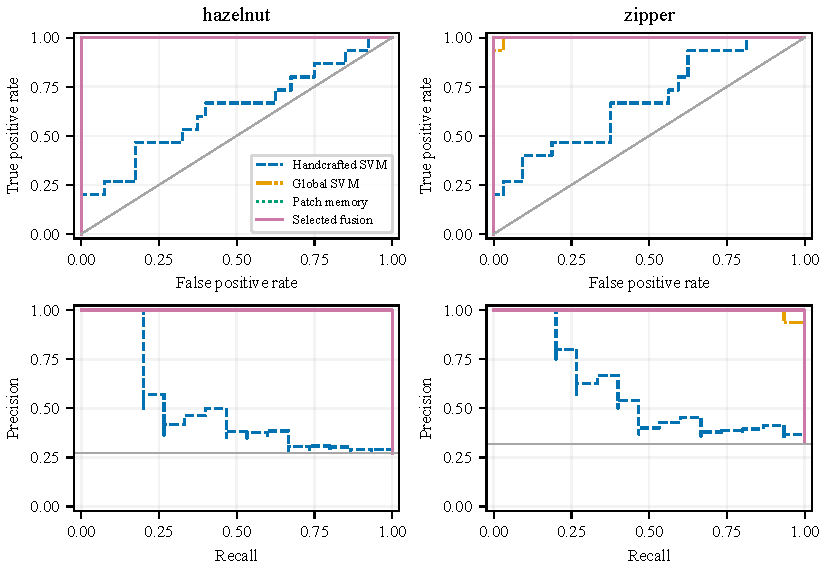
\includegraphics[width=.73\textwidth]{anomaly_curves}
 \caption{测试集的 ROC 和 PR 曲线。PR 图的灰线表示各产品的异常样本比例}
 \Description{The patch and fusion curves overlap at perfect ranking for both products. The handcrafted baseline ranks samples substantially less accurately.}
 \label{fig:anomaly-curves}
\end{figure*}

\subsection{方法}
\textbf{正常图像块最近邻。} 借鉴 PatchCore 的正常图像块记忆库思想\cite{roth2022}。每张训练正常图在每套特征上均匀无放回抽取 64 个位置。记某套训练记忆库为 $B$，查询位置 $u$ 的归一化向量为 $\vect p_u$，其局部分数为
\begin{equation}
 d_u=1-\max_{\vect b\in B}\vect p_u^\top\vect b.
\end{equation}
对 $24\times24$ 网格中的分数排序，取最大的 $\lceil q\cdot576\rceil$ 个求均值。比起对全图平均，只聚合尾部可以保留范围很小的缺陷。两套特征的图像级分数先按训练集折外正常分数的中位数和四分位距进行标准化，再取均值，得到 $s_{\mathrm p}$。局部模型只用正常图构建记忆库，训练异常图用于选择聚合比例。

\textbf{整图分类器。} 用训练集中有标签的正常图和异常图训练径向基核 SVM，采用
$k(\vect z_i,\vect z_j)=\exp(-\gamma\|\vect z_i-\vect z_j\|_2^2)$。
异常类权重为正常类的四倍，以抵消训练样本数量差异。记有符号决策分数为 $s_{\mathrm g}$，正方向对应异常。整图分类器可学习训练集中典型的缺陷响应，正常库分支则反映图像块和已见正常模式的偏离程度。

\textbf{融合与阈值。} 每类做五折分层验证。每折训练使用 160 张正常图与 40 张异常图，验证使用其余 40 张正常图和 10 张异常图。每折每套正常库有 10\,240 个图像块。折外分数来自未使用该训练样本的模型。令 $R(s)=(s-m)/\max(r,10^{-8})$ 表示按正常折外分数的中位数 $m$ 和四分位距 $r$ 缩放。融合分数为
\begin{equation}
 s_c(x)=wR_{\mathrm p}(s_{\mathrm p}(x))+(1-w)R_{\mathrm g}(s_{\mathrm g}(x)).
\end{equation}
候选聚合比例 $q$ 为 1\%、5\% 和 15\%。SVM 的 $C$ 从 $\{0.5,2,8,32\}$ 选择，$\gamma$ 从 $\{0.25,1,4\}$ 选择。融合权重 $w$ 从 0 到 1，以 0.25 为步长枚举。各阶段先比较折均 AUROC，同分时比较折均 AP。最终汇总训练折外分数，选取最大化 $\mathrm{TPR}-\mathrm{FPR}$ 的阈值，同分时用较低阈值。对测试图，分别运行五个折模型并平均各分支分数，使用固定的融合权重和阈值判断。

\begin{table}[tbp]
 \caption{训练集选出的异常检测参数}
 \label{tab:anomaly-parameters}
 \centering
 \begin{tabular}{@{}lrrrrrr@{}}
 \toprule
 产品 & $q$ & $C$ & $\gamma$ & $w$ & $t_c$ & 折均 AUROC \\
 \midrule
 榛子 & 1\% & 8 & 4 & 0.50 & 1.6771 & 1.0000 \\
 拉链 & 15\% & 32 & 4 & 0.50 & 1.4314 & 0.9995 \\
 \bottomrule
 \end{tabular}
\end{table}

表\ref{tab:anomaly-parameters}显示，榛子采用最高的 6 个响应，拉链采用最高的 87 个响应。前者聚焦小面积的强响应，后者汇总更宽范围内的局部变化。训练折参与模型选择，独立测试集用于估计最终效果。若记每套记忆库大小为 $M$，位置数为 $P$，投影维数为 $d$，单次最近邻打分用时 $O(PMd)$，实现分批取最大相似度。

\begin{figure*}[t]
 \centering
 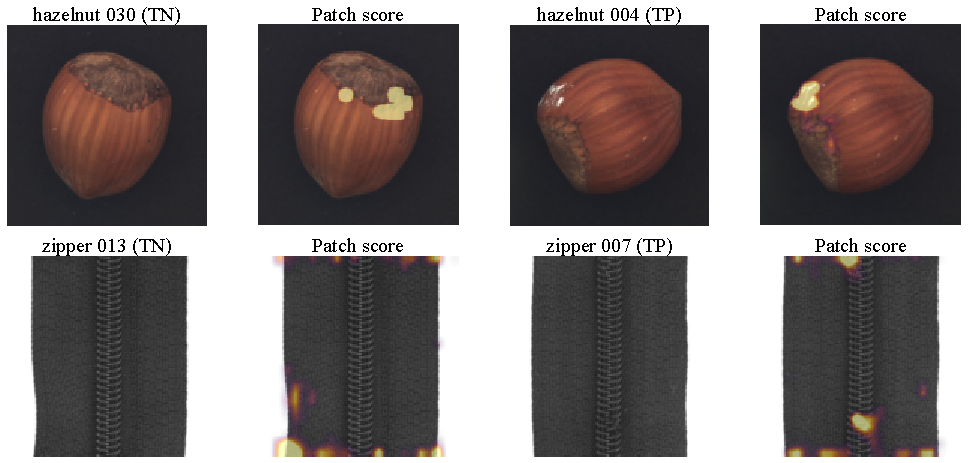
\includegraphics[width=.85\textwidth]{anomaly_examples}
 \caption{各产品距阈值最近的正常图和异常图。热图高亮局部近邻距离较大的区域}
 \Description{Original images and patch-score overlays for hazelnut 030 and 004, and zipper 013 and 007.}
 \label{fig:anomaly-examples}
\end{figure*}

\subsection{实验结果分析}
将异常视为正类。AUROC 衡量异常样本排在正常样本前面的能力，AP 按召回的增量加权各点精确率。固定阈值后报告准确率、精确率、召回率及其调和平均 F1。宏平均是两类指标的等权平均。手工对照使用颜色和灰度差分特征，固定 $C=2$、$\gamma=1$。整图 SVM 和正常图像块模型单独运行，采用各自的训练折外阈值。

\begin{table}[tbp]
 \caption{独立测试集上的异常检测对照}
 \label{tab:anomaly-results}
 \centering
 \begin{tabular}{@{}llrrrr@{}}
 \toprule
 产品 & 方法 & AUROC & AP & ACC & F1 \\
 \midrule
 榛子 & 手工 SVM & .632 & .506 & .291 & .435 \\
      & 整图 SVM & 1.000 & 1.000 & 1.000 & 1.000 \\
      & 正常块近邻 & 1.000 & 1.000 & 1.000 & 1.000 \\
      & 融合 & 1.000 & 1.000 & 1.000 & 1.000 \\
 \addlinespace
 拉链 & 手工 SVM & .683 & .590 & .532 & .500 \\
      & 整图 SVM & .998 & .996 & .979 & .968 \\
      & 正常块近邻 & 1.000 & 1.000 & 1.000 & 1.000 \\
      & 融合 & 1.000 & 1.000 & 1.000 & 1.000 \\
 \addlinespace
 宏平均 & 手工 SVM & .658 & .548 & .411 & .467 \\
      & 整图 SVM & .999 & .998 & .989 & .984 \\
      & 正常块近邻 & 1.000 & 1.000 & 1.000 & 1.000 \\
      & 融合 & 1.000 & 1.000 & 1.000 & 1.000 \\
 \bottomrule
 \end{tabular}
\end{table}

融合模型的混淆计数 $(\mathrm{TN},\mathrm{FP},\mathrm{FN},\mathrm{TP})$ 在榛子上为 $(40,0,0,15)$，在拉链上为 $(32,0,0,15)$，两类精确率与召回率均为 1.000。手工特征丢失了具体缺陷的位置，测试中误报明显增加。拉链的整图模型把正常图 \texttt{032.png} 判为异常，局部模型和融合模型均判为正常。榛子测试集中最高的正常分数为 1.209、最低的异常分数为 2.808，拉链对应为 1.307 和 2.218，两类的训练阈值均位于相应间隔内。融合比两个单分支在训练折上的排序表现略好，与局部模型在独立测试集上并列。曲线重叠见图\ref{fig:anomaly-curves}。

图\ref{fig:anomaly-examples}展示正常与异常图各自最接近阈值的样本。榛子异常图的高响应集中在可见缺陷附近，拉链正常图的边缘也有较强响应。热图在各图内单独归一化，图像间的分数比较使用模型原始输出。测试集中每类只有 15 张异常图。按同一产品内独立同分布的二项模型估计，两类准确率的 95\% Clopper--Pearson 区间分别为 $[0.935,1.000]$ 和 $[0.925,1.000]$。由于当前测试集不存在正负排序颠倒，经验重采样会给出退化的 AUROC 区间，无法反映新批次的不确定性。测试结果覆盖现有产品和成像条件，仍需在新的缺陷类型和光照下复核。



\section{结论}
在课程聚类集上，颜色与纹理已足以把六类产品分开。局部尺度谱聚类给出了同样的划分，五种邻域大小和十次随机初始化的复算结果一致。在异常检测中，整图深度特征和正常图像块分别提供了互补的判断依据。融合模型在训练折上的排序指标最高，并在独立测试集中与局部模型取得相同的满指标结果。对这批图像而言，局部模型也是准确的实现选择。若后续加入新的成像条件或缺陷类型，应重新检查分数分离程度和判定阈值。

\bibliographystyle{ACM-Reference-Format}
\bibliography{course-report-references}
\end{document}

